\documentclass[11pt,]{article}
\usepackage[left=1in,top=1in,right=1in,bottom=1in]{geometry}
\newcommand*{\authorfont}{\fontfamily{phv}\selectfont}
\usepackage[]{mathpazo}


  \usepackage[T1]{fontenc}
  \usepackage[utf8]{inputenc}



\usepackage{abstract}
\renewcommand{\abstractname}{}    % clear the title
\renewcommand{\absnamepos}{empty} % originally center

\renewenvironment{abstract}
 {{%
    \setlength{\leftmargin}{0mm}
    \setlength{\rightmargin}{\leftmargin}%
  }%
  \relax}
 {\endlist}

\makeatletter
\def\@maketitle{%
  \newpage
%  \null
%  \vskip 2em%
%  \begin{center}%
  \let \footnote \thanks
    {\fontsize{18}{20}\selectfont\raggedright  \setlength{\parindent}{0pt} \@title \par}%
}
%\fi
\makeatother




\setcounter{secnumdepth}{3}

\usepackage{color}
\usepackage{fancyvrb}
\newcommand{\VerbBar}{|}
\newcommand{\VERB}{\Verb[commandchars=\\\{\}]}
\DefineVerbatimEnvironment{Highlighting}{Verbatim}{commandchars=\\\{\}}
% Add ',fontsize=\small' for more characters per line
\usepackage{framed}
\definecolor{shadecolor}{RGB}{248,248,248}
\newenvironment{Shaded}{\begin{snugshade}}{\end{snugshade}}
\newcommand{\KeywordTok}[1]{\textcolor[rgb]{0.13,0.29,0.53}{\textbf{#1}}}
\newcommand{\DataTypeTok}[1]{\textcolor[rgb]{0.13,0.29,0.53}{#1}}
\newcommand{\DecValTok}[1]{\textcolor[rgb]{0.00,0.00,0.81}{#1}}
\newcommand{\BaseNTok}[1]{\textcolor[rgb]{0.00,0.00,0.81}{#1}}
\newcommand{\FloatTok}[1]{\textcolor[rgb]{0.00,0.00,0.81}{#1}}
\newcommand{\ConstantTok}[1]{\textcolor[rgb]{0.00,0.00,0.00}{#1}}
\newcommand{\CharTok}[1]{\textcolor[rgb]{0.31,0.60,0.02}{#1}}
\newcommand{\SpecialCharTok}[1]{\textcolor[rgb]{0.00,0.00,0.00}{#1}}
\newcommand{\StringTok}[1]{\textcolor[rgb]{0.31,0.60,0.02}{#1}}
\newcommand{\VerbatimStringTok}[1]{\textcolor[rgb]{0.31,0.60,0.02}{#1}}
\newcommand{\SpecialStringTok}[1]{\textcolor[rgb]{0.31,0.60,0.02}{#1}}
\newcommand{\ImportTok}[1]{#1}
\newcommand{\CommentTok}[1]{\textcolor[rgb]{0.56,0.35,0.01}{\textit{#1}}}
\newcommand{\DocumentationTok}[1]{\textcolor[rgb]{0.56,0.35,0.01}{\textbf{\textit{#1}}}}
\newcommand{\AnnotationTok}[1]{\textcolor[rgb]{0.56,0.35,0.01}{\textbf{\textit{#1}}}}
\newcommand{\CommentVarTok}[1]{\textcolor[rgb]{0.56,0.35,0.01}{\textbf{\textit{#1}}}}
\newcommand{\OtherTok}[1]{\textcolor[rgb]{0.56,0.35,0.01}{#1}}
\newcommand{\FunctionTok}[1]{\textcolor[rgb]{0.00,0.00,0.00}{#1}}
\newcommand{\VariableTok}[1]{\textcolor[rgb]{0.00,0.00,0.00}{#1}}
\newcommand{\ControlFlowTok}[1]{\textcolor[rgb]{0.13,0.29,0.53}{\textbf{#1}}}
\newcommand{\OperatorTok}[1]{\textcolor[rgb]{0.81,0.36,0.00}{\textbf{#1}}}
\newcommand{\BuiltInTok}[1]{#1}
\newcommand{\ExtensionTok}[1]{#1}
\newcommand{\PreprocessorTok}[1]{\textcolor[rgb]{0.56,0.35,0.01}{\textit{#1}}}
\newcommand{\AttributeTok}[1]{\textcolor[rgb]{0.77,0.63,0.00}{#1}}
\newcommand{\RegionMarkerTok}[1]{#1}
\newcommand{\InformationTok}[1]{\textcolor[rgb]{0.56,0.35,0.01}{\textbf{\textit{#1}}}}
\newcommand{\WarningTok}[1]{\textcolor[rgb]{0.56,0.35,0.01}{\textbf{\textit{#1}}}}
\newcommand{\AlertTok}[1]{\textcolor[rgb]{0.94,0.16,0.16}{#1}}
\newcommand{\ErrorTok}[1]{\textcolor[rgb]{0.64,0.00,0.00}{\textbf{#1}}}
\newcommand{\NormalTok}[1]{#1}

\usepackage{graphicx,grffile}
\makeatletter
\def\maxwidth{\ifdim\Gin@nat@width>\linewidth\linewidth\else\Gin@nat@width\fi}
\def\maxheight{\ifdim\Gin@nat@height>\textheight\textheight\else\Gin@nat@height\fi}
\makeatother
% Scale images if necessary, so that they will not overflow the page
% margins by default, and it is still possible to overwrite the defaults
% using explicit options in \includegraphics[width, height, ...]{}
\setkeys{Gin}{width=\maxwidth,height=\maxheight,keepaspectratio}

\title{Mi proyecto :Datos Puntuales Superficie Continua y Creación de Isolíneas
en R (Mapas de Precipitación).\\
Trabajo :Proyecto Final de Analis Espacial\\
Profesor :Jose Ramon Martinez Batlle  }



\author{\Large Adalberto Guerrero P.\vspace{0.05in} \newline\normalsize\emph{Estudiante, Universidad Autónoma de Santo Domingo (UASD)}  }


\date{}

\usepackage{titlesec}

\titleformat*{\section}{\normalsize\bfseries}
\titleformat*{\subsection}{\normalsize\itshape}
\titleformat*{\subsubsection}{\normalsize\itshape}
\titleformat*{\paragraph}{\normalsize\itshape}
\titleformat*{\subparagraph}{\normalsize\itshape}

\titlespacing{\section}
{0pt}{36pt}{0pt}
\titlespacing{\subsection}
{0pt}{36pt}{0pt}
\titlespacing{\subsubsection}
{0pt}{36pt}{0pt}





\newtheorem{hypothesis}{Hypothesis}
\usepackage{setspace}

\makeatletter
\@ifpackageloaded{hyperref}{}{%
\ifxetex
  \PassOptionsToPackage{hyphens}{url}\usepackage[setpagesize=false, % page size defined by xetex
              unicode=false, % unicode breaks when used with xetex
              xetex]{hyperref}
\else
  \PassOptionsToPackage{hyphens}{url}\usepackage[unicode=true]{hyperref}
\fi
}

\@ifpackageloaded{color}{
    \PassOptionsToPackage{usenames,dvipsnames}{color}
}{%
    \usepackage[usenames,dvipsnames]{color}
}
\makeatother
\hypersetup{breaklinks=true,
            bookmarks=true,
            pdfauthor={Adalberto Guerrero P. (Estudiante, Universidad Autónoma de Santo Domingo (UASD))},
             pdfkeywords = {Isoyetas, pluviometros},  
            pdftitle={Mi proyecto :Datos Puntuales Superficie Continua y Creación de Isolíneas
en R (Mapas de Precipitación).\\
Trabajo :Proyecto Final de Analis Espacial\\
Profesor :Jose Ramon Martinez Batlle},
            colorlinks=true,
            citecolor=blue,
            urlcolor=blue,
            linkcolor=magenta,
            pdfborder={0 0 0}}
\urlstyle{same}  % don't use monospace font for urls

% set default figure placement to htbp
\makeatletter
\def\fps@figure{htbp}
\makeatother

\usepackage{pdflscape} \newcommand{\blandscape}{\begin{landscape}}
\newcommand{\elandscape}{\end{landscape}}


% add tightlist ----------
\providecommand{\tightlist}{%
\setlength{\itemsep}{0pt}\setlength{\parskip}{0pt}}

\begin{document}
	
% \pagenumbering{arabic}% resets `page` counter to 1 
%
% \maketitle

{% \usefont{T1}{pnc}{m}{n}
\setlength{\parindent}{0pt}
\thispagestyle{plain}
{\fontsize{18}{20}\selectfont\raggedright 
\maketitle  % title \par  

}

{
   \vskip 13.5pt\relax \normalsize\fontsize{11}{12} 
\textbf{\authorfont Adalberto Guerrero P.} \hskip 15pt \emph{\small Estudiante, Universidad Autónoma de Santo Domingo (UASD)}   

}

}








\begin{abstract}

    \hbox{\vrule height .2pt width 39.14pc}

    \vskip 8.5pt % \small 

\noindent Mi resumen


\vskip 8.5pt \noindent \emph{Keywords}: Isoyetas, pluviometros \par

    \hbox{\vrule height .2pt width 39.14pc}



\end{abstract}


\vskip 6.5pt


\noindent  \section{Introducción}\label{introducciuxf3n}

El presente proyecto se trata de generar una superficie continua y
atraves de ella crear un mapa de isoyetas, para esto utilizaremos la
capa de provincias de la OFICINA NACIONAL DE ESTADISTICA (ONE) y los
datos de lluvia de la OFICINA NACIONAL DE METEOROLOGIA (ONAMET) los
datos de lluvia corresponden al año 1998, año en el cual fuimos
golpeados por un fenomeno meteorologico muy fuerte qeu causo muchos
daños al pais, causo inundaciones en casi en todo el territorio nacional
asi como grandes areas de bosques y cutivos debastadas, debido a sus
fuertes vientos. el nombre de este fenomeno es el Ciclon GEORGE. en el
pais ocurrieron muchas lluvias durante casi todo el año 1998.es por esta
razon nuestro interes de realizar el analisis para este tiempo.

\section{Metodología}\label{metodologuxeda}

Segun la orientacion del profesor jose ramon martinez batlle. para
realizar este proyecto primero debemos generar una superficie continua
usando los datos de lluvia y la capa de provincia y combinando las
diferentes lineas de codigos aprendidas durante el desarrollo de esta
materia. al final para general el mapa de isoyetas bastara con ejecutar
el paquete contour data. disponible para R. y realisar algunos ajustes
para la presentacion del mapa.

\ldots

\subsection{Paquetes}\label{paquetes}

\begin{itemize}
\tightlist
\item
  Carga el paquete \texttt{sf}, la colección \texttt{tidyverse} y los
  paquetes \texttt{spdep}, \texttt{lmtest}, \texttt{tmap} y
  \texttt{RColorBrewer}
\end{itemize}

\begin{Shaded}
\begin{Highlighting}[]
\KeywordTok{library}\NormalTok{(sf)}
\end{Highlighting}
\end{Shaded}

\begin{verbatim}
## Linking to GEOS 3.7.1, GDAL 2.4.2, PROJ 5.2.0
\end{verbatim}

\begin{Shaded}
\begin{Highlighting}[]
\KeywordTok{library}\NormalTok{(tidyverse)}
\end{Highlighting}
\end{Shaded}

\begin{verbatim}
## -- Attaching packages ------------------------------------------------ tidyverse 1.2.1 --
\end{verbatim}

\begin{verbatim}
## v ggplot2 3.2.1     v purrr   0.3.3
## v tibble  2.1.3     v dplyr   0.8.3
## v tidyr   1.0.0     v stringr 1.4.0
## v readr   1.3.1     v forcats 0.4.0
\end{verbatim}

\begin{verbatim}
## -- Conflicts --------------------------------------------------- tidyverse_conflicts() --
## x dplyr::filter() masks stats::filter()
## x dplyr::lag()    masks stats::lag()
\end{verbatim}

\begin{Shaded}
\begin{Highlighting}[]
\KeywordTok{library}\NormalTok{(spdep)}
\end{Highlighting}
\end{Shaded}

\begin{verbatim}
## Loading required package: sp
\end{verbatim}

\begin{verbatim}
## Loading required package: spData
\end{verbatim}

\begin{verbatim}
## To access larger datasets in this package, install the spDataLarge
## package with: `install.packages('spDataLarge',
## repos='https://nowosad.github.io/drat/', type='source')`
\end{verbatim}

\begin{Shaded}
\begin{Highlighting}[]
\KeywordTok{library}\NormalTok{(lmtest)}
\end{Highlighting}
\end{Shaded}

\begin{verbatim}
## Loading required package: zoo
\end{verbatim}

\begin{verbatim}
## 
## Attaching package: 'zoo'
\end{verbatim}

\begin{verbatim}
## The following objects are masked from 'package:base':
## 
##     as.Date, as.Date.numeric
\end{verbatim}

\begin{Shaded}
\begin{Highlighting}[]
\KeywordTok{library}\NormalTok{(tmap)}
\KeywordTok{library}\NormalTok{(RColorBrewer)}
\KeywordTok{library}\NormalTok{(gstat)}
\end{Highlighting}
\end{Shaded}

\begin{verbatim}
## Registered S3 method overwritten by 'xts':
##   method     from
##   as.zoo.xts zoo
\end{verbatim}

\subsection{Cargar Datos}\label{cargar-datos}

\begin{Shaded}
\begin{Highlighting}[]
\NormalTok{rutapre <-}\StringTok{ 'material-de-apoyo-master/data/onamet_prec_anual_sf.gpkg'}
\NormalTok{rutadiv <-}\StringTok{ 'material-de-apoyo-master/data/divisionRD.gpkg'}
\NormalTok{pre <-}\StringTok{ }\KeywordTok{st_read}\NormalTok{(rutapre)}
\end{Highlighting}
\end{Shaded}

\begin{verbatim}
## Reading layer `onamet_prec_anual_sf' from data source `/home/franc/unidad-0-asignacion-99-mi-proyecto-Adalbertogp2020/material-de-apoyo-master/data/onamet_prec_anual_sf.gpkg' using driver `GPKG'
## Simple feature collection with 25 features and 37 fields
## geometry type:  POINT
## dimension:      XY
## bbox:           xmin: -71.7 ymin: 18.067 xmax: -68.367 ymax: 19.85
## epsg (SRID):    4326
## proj4string:    +proj=longlat +datum=WGS84 +no_defs
\end{verbatim}

\begin{Shaded}
\begin{Highlighting}[]
\NormalTok{prov <-}\StringTok{ }\KeywordTok{st_read}\NormalTok{(rutadiv, }\DataTypeTok{layer =} \StringTok{'PROVCenso2010'}\NormalTok{)}
\end{Highlighting}
\end{Shaded}

\begin{verbatim}
## Reading layer `PROVCenso2010' from data source `/home/franc/unidad-0-asignacion-99-mi-proyecto-Adalbertogp2020/material-de-apoyo-master/data/divisionRD.gpkg' using driver `GPKG'
## Simple feature collection with 32 features and 4 fields
## geometry type:  MULTIPOLYGON
## dimension:      XY
## bbox:           xmin: 182215.8 ymin: 1933532 xmax: 571365.3 ymax: 2205216
## epsg (SRID):    32619
## proj4string:    +proj=utm +zone=19 +datum=WGS84 +units=m +no_defs
\end{verbatim}

\subsection{Transformar Datos.}\label{transformar-datos.}

\begin{Shaded}
\begin{Highlighting}[]
\KeywordTok{st_crs}\NormalTok{(pre)}
\end{Highlighting}
\end{Shaded}

\begin{verbatim}
## Coordinate Reference System:
##   EPSG: 4326 
##   proj4string: "+proj=longlat +datum=WGS84 +no_defs"
\end{verbatim}

\begin{Shaded}
\begin{Highlighting}[]
\NormalTok{crsdestino <-}\StringTok{ }\DecValTok{32619}
\NormalTok{preutm <-}\StringTok{ }\NormalTok{pre }\OperatorTok\StringTok{ }\KeywordTok{st_transform}\NormalTok{(}\DataTypeTok{crs =}\NormalTok{ crsdestino)}
\NormalTok{preutm}
\end{Highlighting}
\end{Shaded}

\begin{verbatim}
## Simple feature collection with 25 features and 37 fields
## geometry type:  POINT
## dimension:      XY
## bbox:           xmin: 215264.1 ymin: 1999092 xmax: 566794.7 ymax: 2197035
## epsg (SRID):    32619
## proj4string:    +proj=utm +zone=19 +datum=WGS84 +units=m +no_defs
## First 10 features:
##            Estación  a1979  a1980  a1981  a1982  a1983  a1984  a1985
## 1          Barahona 1740.0 1053.6 1435.3  815.3 1183.0  584.1  997.8
## 2         Bayaguana 2794.3 1761.5 2412.4 1758.6 1857.1 1645.6 1928.3
## 3           Cabrera 2035.0 1276.8     NA 2136.9 1703.8 1888.7 1557.1
## 4         Constanza 1652.1 1166.9 1343.3  921.2  828.4     NA  892.8
## 5  Gaspar Hernández     NA 1443.8 2174.9 1844.1 1688.8 2208.8 1895.5
## 6       Hondo Valle 1823.6 1778.2 2203.7 1709.9 1841.3 1796.6 1309.5
## 7            Jimaní 1060.7  639.1  960.2  507.5  610.7  641.5  689.6
## 8          La Unión 1781.5 1630.6 2304.4 1413.1 1288.4 1499.4 1157.1
## 9           La Vega 1833.5 1304.3 1993.7 1483.2 1353.9 1550.1 1084.9
## 10     Las Américas 1958.4  958.7 1513.4  787.4  975.5  954.9 1398.2
##     a1986  a1987  a1988  a1989   a1990  a1991  a1992  a1993  a1994   a1995
## 1  1080.0 1423.9  704.7 1011.6 1075.20  983.1 1112.5  968.5 1622.4  956.00
## 2  2182.2 2273.5 1813.2 1730.6 1823.40 1850.3 1765.7 1606.2 1892.8 1360.10
## 3  1597.0 2059.7     NA 1176.9 1183.40  957.6     NA     NA     NA      NA
## 4   715.8  786.9  837.7  671.5  875.35     NA  858.6  858.6  900.7  839.40
## 5  2874.7 2360.8 1426.3 1214.2 1530.70     NA 1257.5 1345.3 1824.9 1665.45
## 6  1589.7 1778.8 1766.5 1722.8 1596.10 1088.4 1731.0 1887.0 1772.0 1288.30
## 7   802.4  648.9  521.0  680.7  880.00  311.6  809.2  472.9  840.2  909.00
## 8  1313.1 1786.5 1888.8 1222.8 1808.00 1250.4 1555.2 1484.8 1035.9  877.70
## 9  1767.1 1663.2 1934.9 1192.4 1664.40 1146.4 1565.6 1855.4 1455.7 1175.40
## 10 1419.0 1866.4 1620.5 1151.7      NA  997.0     NA     NA     NA 1017.50
##      a1996   a1997  a1998  a1999  a2000  a2001  a2002   a2003  a2004
## 1   965.65  662.60  684.6  662.7  600.0  600.0  997.6  942.60  972.6
## 2  1867.70 1618.60 2156.6 1712.5 1868.5 1796.1 1658.0 2117.30 1554.2
## 3       NA      NA     NA     NA 1538.6 1852.9  946.9 1810.95 2053.3
## 4  1167.30  525.10 1492.7 1077.8  951.3  787.1  959.2 1084.10  985.9
## 5  2656.80  984.80 2147.9 1791.9 1716.9 2178.8 1093.4 2058.50 1906.8
## 6  1447.90  912.65 1813.9 1762.2 2285.9 1604.3 1477.4 1628.10 1617.7
## 7   816.20  358.20  824.1 1037.0  833.9  488.4  510.1  656.70  866.9
## 8  1980.50  554.20 1744.1 1314.3 1148.5 1360.5  972.1 1802.00 2550.1
## 9  1772.50 1018.80 1549.6 1817.9 1368.6 1522.0 1200.7 2290.60 1825.7
## 10 1019.60  651.20 1218.6 1125.9  809.7  747.6  933.4 1083.60 1338.9
##      a2005   a2006   a2007   a2008  a2009  a2010  a2011  a2012  a2013
## 1  1274.60 1118.40 1531.30 1136.80  583.3 1036.3 1280.2 1726.3  576.2
## 2  2102.80 2097.10 2137.60 1831.20 1607.9 1881.6 1849.9 2350.8 2108.0
## 3  1451.10 1957.90      NA      NA     NA 2411.4 1920.1 2821.3     NA
## 4  1245.20 1162.20 1661.40 1072.90  902.8 1024.5 1008.2 1188.1 1016.3
## 5  2001.85 1992.00 3282.65 1866.30 2386.1 2639.2 1727.2 2524.0 1448.2
## 6  1554.65 1487.15 1487.15 1399.15 1461.9 2005.6 1309.0 1736.8 1390.2
## 7   929.30  963.90 1084.00  751.10  694.9  807.1  879.5 1037.3  292.9
## 8  2034.30 2106.60 2764.80 1536.30 1605.8 2255.6 1719.2 2484.3 1299.2
## 9  1245.20 1162.20 1661.40 1072.90 2867.4 1486.4 1434.1 2204.7 1227.0
## 10 1744.60 1141.70 1457.50 1718.40 1369.1 2422.4 1885.5 1658.7 1039.6
##     a2014                     geom
## 1   845.9 POINT (277900.2 2013585)
## 2  1505.6 POINT (433242.1 2073284)
## 3  1975.6   POINT (405636 2171119)
## 4   764.1 POINT (320947.7 2090623)
## 5  1928.7 POINT (363678.2 2169619)
## 6   908.9 POINT (215264.1 2071669)
## 7   502.0 POINT (221953.7 2045651)
## 8  1741.5 POINT (337592.1 2184559)
## 9  1812.5 POINT (338847.1 2125548)
## 10  909.4 POINT (429562.7 2038222)
\end{verbatim}

\subsection{EDA básico}\label{eda-buxe1sico}

ahora vamos a construir los datos para el año 1998:

\begin{Shaded}
\begin{Highlighting}[]
\KeywordTok{nrow}\NormalTok{(preutm)}
\end{Highlighting}
\end{Shaded}

\begin{verbatim}
## [1] 25
\end{verbatim}

\begin{Shaded}
\begin{Highlighting}[]
\KeywordTok{summary}\NormalTok{(preutm}\OperatorTok{$}\NormalTok{a1998)}
\end{Highlighting}
\end{Shaded}

\begin{verbatim}
##    Min. 1st Qu.  Median    Mean 3rd Qu.    Max.    NA's 
##   684.6  1151.7  1580.5  1644.0  1987.7  3011.3       2
\end{verbatim}

\begin{Shaded}
\begin{Highlighting}[]
\KeywordTok{hist}\NormalTok{(preutm}\OperatorTok{$}\NormalTok{a1998)}
\end{Highlighting}
\end{Shaded}

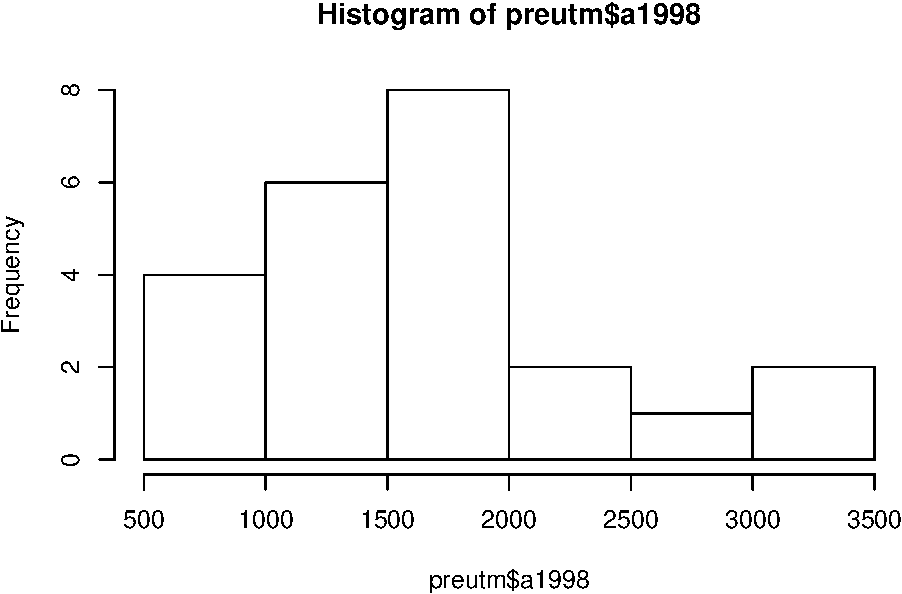
\includegraphics{proyecto_Superficie_Continua_files/figure-latex/unnamed-chunk-4-1.pdf}

\begin{Shaded}
\begin{Highlighting}[]
\KeywordTok{hist}\NormalTok{(}\KeywordTok{log}\NormalTok{(preutm}\OperatorTok{$}\NormalTok{a1998))}
\end{Highlighting}
\end{Shaded}

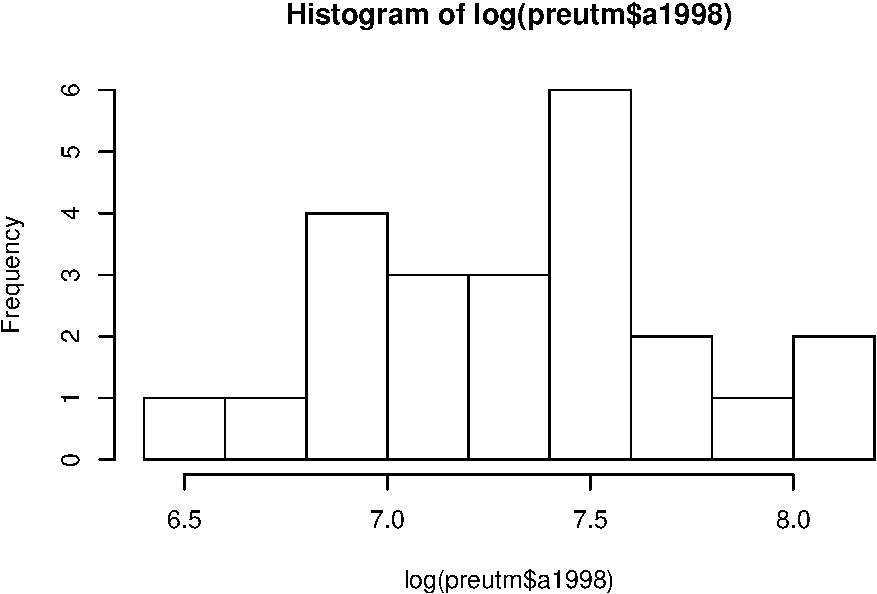
\includegraphics{proyecto_Superficie_Continua_files/figure-latex/unnamed-chunk-4-2.pdf}

\begin{Shaded}
\begin{Highlighting}[]
\KeywordTok{shapiro.test}\NormalTok{(preutm}\OperatorTok{$}\NormalTok{a1998)}
\end{Highlighting}
\end{Shaded}

\begin{verbatim}
## 
##  Shapiro-Wilk normality test
## 
## data:  preutm$a1998
## W = 0.94806, p-value = 0.2666
\end{verbatim}

\begin{Shaded}
\begin{Highlighting}[]
\KeywordTok{shapiro.test}\NormalTok{(}\KeywordTok{log}\NormalTok{(pre}\OperatorTok{$}\NormalTok{a1998))}
\end{Highlighting}
\end{Shaded}

\begin{verbatim}
## 
##  Shapiro-Wilk normality test
## 
## data:  log(pre$a1998)
## W = 0.97788, p-value = 0.8671
\end{verbatim}

Segun el histograma los datos siguen distribución normal para la
variable modificada, Igualmente, de los 25 pluviometros que teniamos en
el pais para le año 1998 hay dos con datos perdidos (NA). Eliminemos
dichos datos, y crearemos solo los obejtos de 1998 que tengan datos:

\begin{Shaded}
\begin{Highlighting}[]
\NormalTok{pre1998 <-}\StringTok{ }\KeywordTok{na.omit}\NormalTok{(preutm[,}\KeywordTok{c}\NormalTok{(}\StringTok{'Estación', '}\NormalTok{a1998}\StringTok{')])}
\StringTok{pre1998$a1998log <- log(pre1998$a1998)}
\StringTok{pre1998}
\end{Highlighting}
\end{Shaded}

\begin{verbatim}
## Simple feature collection with 23 features and 3 fields
## geometry type:  POINT
## dimension:      XY
## bbox:           xmin: 215264.1 ymin: 1999092 xmax: 566794.7 ymax: 2197035
## epsg (SRID):    32619
## proj4string:    +proj=utm +zone=19 +datum=WGS84 +units=m +no_defs
## First 10 features:
##            Estación  a1998                     geom a1998log
## 1          Barahona  684.6 POINT (277900.2 2013585) 6.528835
## 2         Bayaguana 2156.6 POINT (433242.1 2073284) 7.676288
## 4         Constanza 1492.7 POINT (320947.7 2090623) 7.308342
## 5  Gaspar Hernández 2147.9 POINT (363678.2 2169619) 7.672246
## 6       Hondo Valle 1813.9 POINT (215264.1 2071669) 7.503235
## 7            Jimaní  824.1 POINT (221953.7 2045651) 6.714292
## 8          La Unión 1744.1 POINT (337592.1 2184559) 7.463994
## 9           La Vega 1549.6 POINT (338847.1 2125548) 7.345752
## 10     Las Américas 1218.6 POINT (429562.7 2038222) 7.105458
## 11             Moca 1036.4 POINT (342475.8 2143891) 6.943508
\end{verbatim}

\section{Visualizamos los observatorios, ya depurados según la
precipitación del año
1998:}\label{visualizamos-los-observatorios-ya-depurados-seguxfan-la-precipitaciuxf3n-del-auxf1o-1998}

\begin{Shaded}
\begin{Highlighting}[]
\KeywordTok{library}\NormalTok{(ggplot2)}
\KeywordTok{ggplot}\NormalTok{() }\OperatorTok{+}
\StringTok{  }\KeywordTok{geom_sf}\NormalTok{(}\DataTypeTok{data =}\NormalTok{ prov, }\DataTypeTok{fill =} \StringTok{'white'}\NormalTok{) }\OperatorTok{+}
\StringTok{  }\KeywordTok{geom_sf}\NormalTok{(}\DataTypeTok{data =}\NormalTok{ pre1998, }\KeywordTok{aes}\NormalTok{(}\DataTypeTok{col =}\NormalTok{ a1998log), }\DataTypeTok{size =} \DecValTok{6}\NormalTok{) }\OperatorTok{+}
\StringTok{  }\KeywordTok{scale_colour_gradient}\NormalTok{(}\DataTypeTok{low=}\StringTok{"#deebf7"}\NormalTok{, }\DataTypeTok{high=}\StringTok{"#3182bd"}\NormalTok{) }\OperatorTok{+}
\StringTok{  }\KeywordTok{geom_sf_text}\NormalTok{(}\DataTypeTok{data =}\NormalTok{ prov, }\KeywordTok{aes}\NormalTok{(}\DataTypeTok{label=}\NormalTok{TOPONIMIA), }\DataTypeTok{check_overlap =}\NormalTok{ T, }\DataTypeTok{size =} \DecValTok{2}\NormalTok{) }\OperatorTok{+}
\StringTok{  }\KeywordTok{geom_sf_text}\NormalTok{(}\DataTypeTok{data =}\NormalTok{ pre1998, }\KeywordTok{aes}\NormalTok{(}\DataTypeTok{label=}\NormalTok{Estación), }\DataTypeTok{check_overlap =}\NormalTok{ T, }\DataTypeTok{size =} \FloatTok{1.5}\NormalTok{) }\OperatorTok{+}
\StringTok{  }\KeywordTok{theme_bw}\NormalTok{()}
\end{Highlighting}
\end{Shaded}

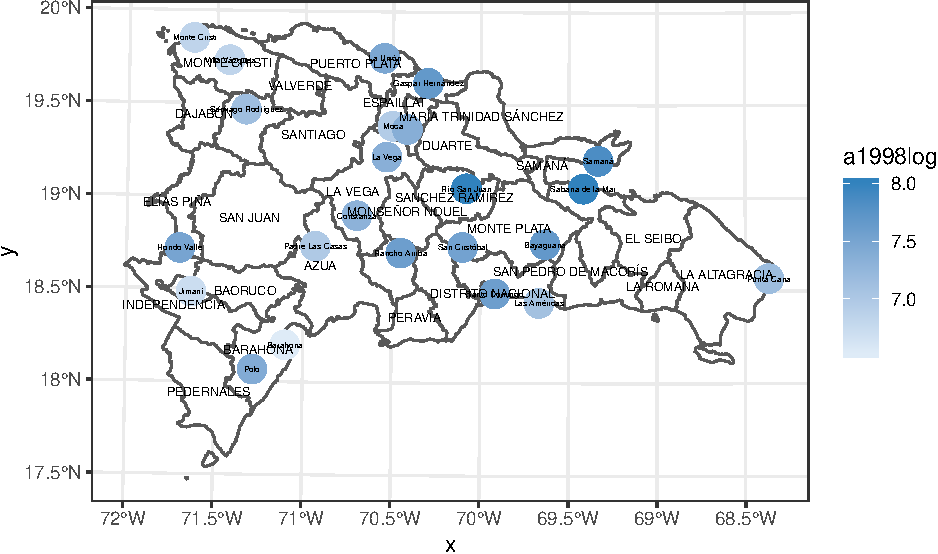
\includegraphics{proyecto_Superficie_Continua_files/figure-latex/unnamed-chunk-6-1.pdf}

\subsection{Variograma muestral}\label{variograma-muestral}

Crearemos el variograma muestral para la variable modificada de la
precipitación o sea la parte logaritmica.

\begin{Shaded}
\begin{Highlighting}[]
\NormalTok{f98 <-}\StringTok{ }\KeywordTok{variogram}\NormalTok{(a1998log}\OperatorTok{~}\DecValTok{1}\NormalTok{, pre1998)}
\NormalTok{f98}
\end{Highlighting}
\end{Shaded}

\begin{verbatim}
##    np       dist      gamma dir.hor dir.ver   id
## 1   1   8896.559 0.08905032       0       0 var1
## 2   6  22368.506 0.13141962       0       0 var1
## 3  10  32110.478 0.08693293       0       0 var1
## 4   6  40706.420 0.03361319       0       0 var1
## 5   6  50780.415 0.12041650       0       0 var1
## 6  12  58446.995 0.10567299       0       0 var1
## 7   8  67239.009 0.06443833       0       0 var1
## 8   7  77115.401 0.11793609       0       0 var1
## 9  17  85657.115 0.15764350       0       0 var1
## 10 12  93304.363 0.11849679       0       0 var1
## 11  7 103800.452 0.02103140       0       0 var1
## 12 19 112257.676 0.11604918       0       0 var1
## 13 16 120305.537 0.21044124       0       0 var1
## 14 12 128383.382 0.15380975       0       0 var1
\end{verbatim}

\begin{Shaded}
\begin{Highlighting}[]
\KeywordTok{plot}\NormalTok{(f98, }\DataTypeTok{plot.numbers =}\NormalTok{ T)}
\end{Highlighting}
\end{Shaded}

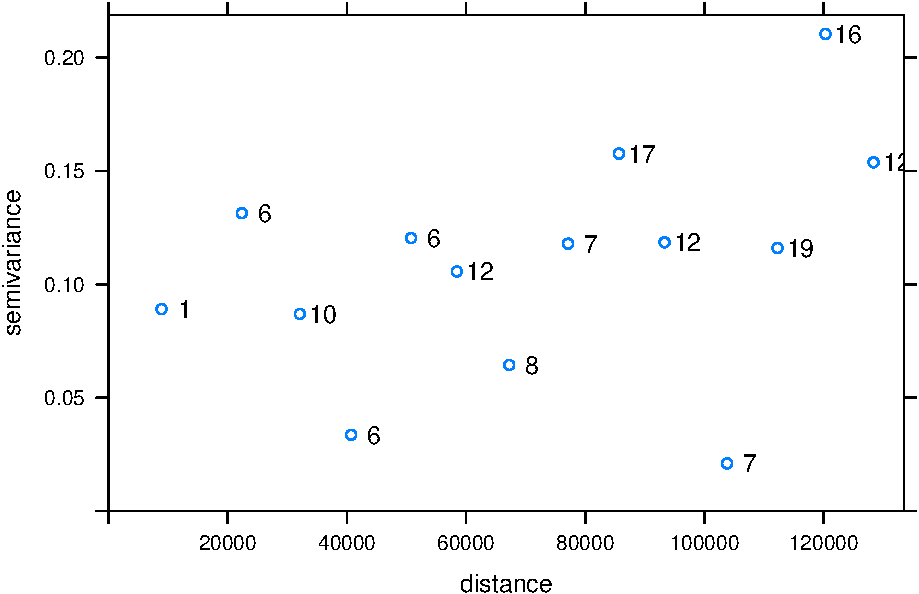
\includegraphics{proyecto_Superficie_Continua_files/figure-latex/unnamed-chunk-7-1.pdf}

\subsection{Variograma modelo.}\label{variograma-modelo.}

Después de construir el variograma muestral, vamos a construir un
variograma modelo para esto utilizaremos la funcios Krige para
interpolar los datos.

\begin{Shaded}
\begin{Highlighting}[]
\NormalTok{f98_m <-}\StringTok{ }\KeywordTok{fit.variogram}\NormalTok{(f98, }\KeywordTok{vgm}\NormalTok{(}\DataTypeTok{model =} \StringTok{"Sph"}\NormalTok{, }\DataTypeTok{range =} \DecValTok{50000}\NormalTok{))}
\NormalTok{f98_m}
\end{Highlighting}
\end{Shaded}

\begin{verbatim}
##   model     psill    range
## 1   Sph 0.1078617 13982.71
\end{verbatim}

\begin{Shaded}
\begin{Highlighting}[]
\KeywordTok{plot}\NormalTok{(f98, f98_m, }\DataTypeTok{plot.numbers =}\NormalTok{ T)}
\end{Highlighting}
\end{Shaded}

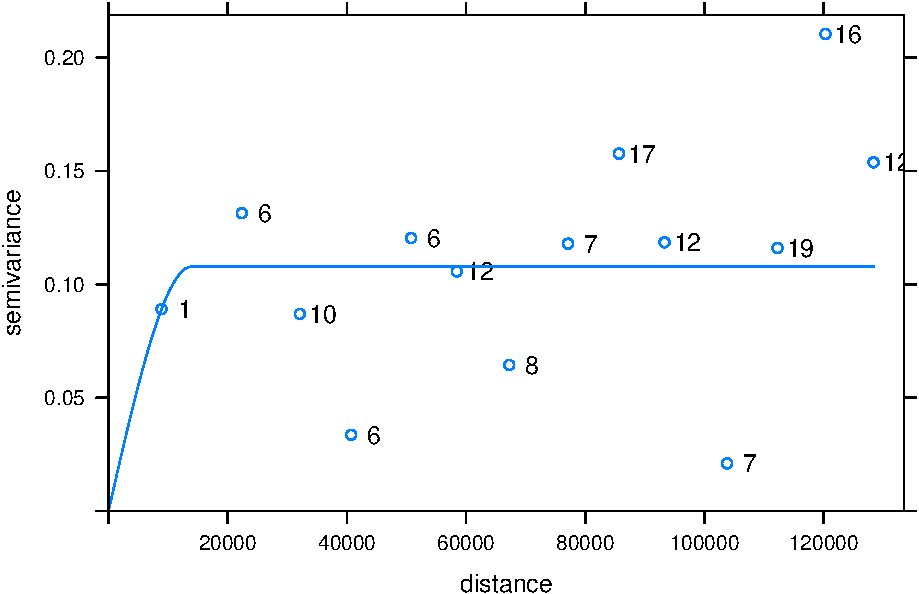
\includegraphics{proyecto_Superficie_Continua_files/figure-latex/unnamed-chunk-8-1.pdf}

\begin{Shaded}
\begin{Highlighting}[]
\NormalTok{f98_m2 <-}\StringTok{ }\KeywordTok{fit.variogram}\NormalTok{(f98, }\KeywordTok{vgm}\NormalTok{(}\DataTypeTok{model =} \StringTok{"Exp"}\NormalTok{, }\DataTypeTok{range =} \DecValTok{50000}\NormalTok{))}
\NormalTok{f98_m2}
\end{Highlighting}
\end{Shaded}

\begin{verbatim}
##   model     psill    range
## 1   Exp 0.1073634 4605.641
\end{verbatim}

\begin{Shaded}
\begin{Highlighting}[]
\KeywordTok{plot}\NormalTok{(f98, f98_m2, }\DataTypeTok{plot.numbers =}\NormalTok{ T)}
\end{Highlighting}
\end{Shaded}

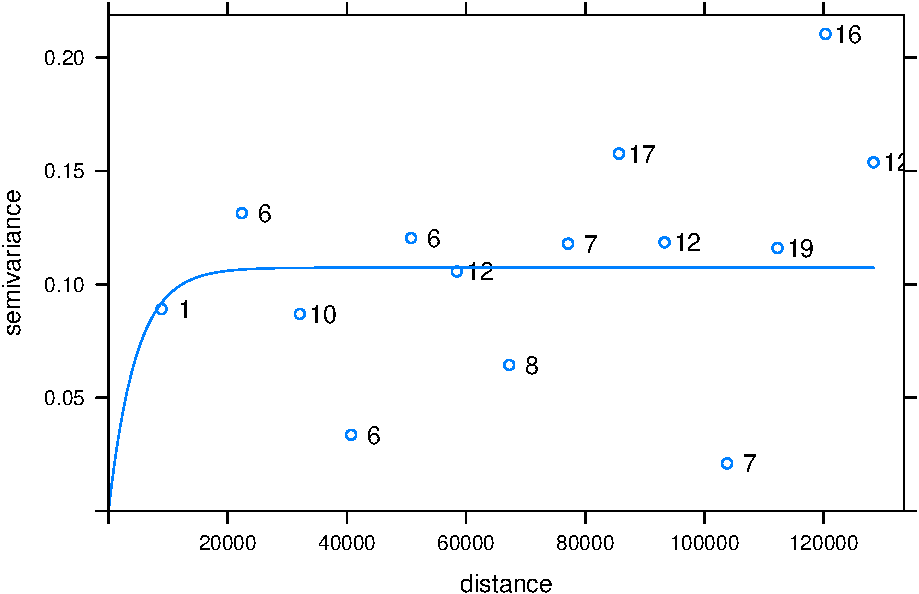
\includegraphics{proyecto_Superficie_Continua_files/figure-latex/unnamed-chunk-8-2.pdf}

\begin{Shaded}
\begin{Highlighting}[]
\NormalTok{f98_m3 <-}\StringTok{ }\KeywordTok{fit.variogram}\NormalTok{(f98, }\KeywordTok{vgm}\NormalTok{(}\DataTypeTok{model =} \StringTok{"Gau"}\NormalTok{, }\DataTypeTok{range =} \DecValTok{50000}\NormalTok{))}
\end{Highlighting}
\end{Shaded}

\begin{verbatim}
## Warning in fit.variogram(f98, vgm(model = "Gau", range = 50000)): No
## convergence after 200 iterations: try different initial values?
\end{verbatim}

\begin{Shaded}
\begin{Highlighting}[]
\NormalTok{f98_m3}
\end{Highlighting}
\end{Shaded}

\begin{verbatim}
##   model     psill   range
## 1   Gau 0.1078316 5250.27
\end{verbatim}

\begin{Shaded}
\begin{Highlighting}[]
\KeywordTok{plot}\NormalTok{(f98, f98_m3, }\DataTypeTok{plot.numbers =}\NormalTok{ T)}
\end{Highlighting}
\end{Shaded}

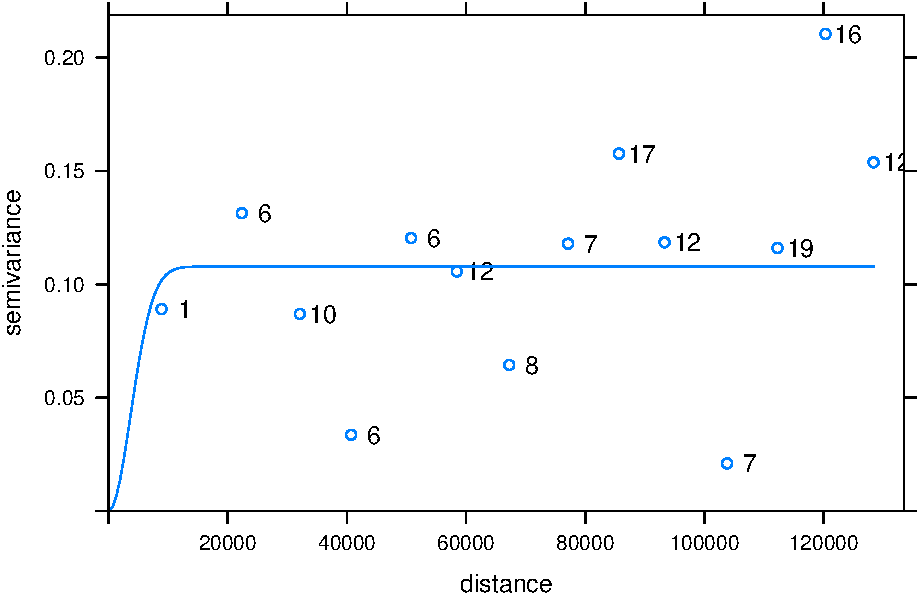
\includegraphics{proyecto_Superficie_Continua_files/figure-latex/unnamed-chunk-8-3.pdf}

\begin{Shaded}
\begin{Highlighting}[]
\KeywordTok{attr}\NormalTok{(f98_m, }\StringTok{'SSErr'}\NormalTok{)}
\end{Highlighting}
\end{Shaded}

\begin{verbatim}
## [1] 5.877132e-11
\end{verbatim}

\begin{Shaded}
\begin{Highlighting}[]
\KeywordTok{attr}\NormalTok{(f98_m2, }\StringTok{'SSErr'}\NormalTok{) }
\end{Highlighting}
\end{Shaded}

\begin{verbatim}
## [1] 5.93196e-11
\end{verbatim}

\begin{Shaded}
\begin{Highlighting}[]
\KeywordTok{attr}\NormalTok{(f98_m3, }\StringTok{'SSErr'}\NormalTok{)}
\end{Highlighting}
\end{Shaded}

\begin{verbatim}
## [1] 6.080129e-11
\end{verbatim}

\subsection{Interpolación por kriging
ordinario}\label{interpolaciuxf3n-por-kriging-ordinario}

Para esta interpolacion crearemos una cuadrícula con las
precipitaciones. una cuadrícula apropiada para RD,seria una de baja
resolución, por ejemplo 1x1km:

\begin{Shaded}
\begin{Highlighting}[]
\KeywordTok{library}\NormalTok{(stars)}
\end{Highlighting}
\end{Shaded}

\begin{verbatim}
## Loading required package: abind
\end{verbatim}

\begin{Shaded}
\begin{Highlighting}[]
\NormalTok{grd <-}\StringTok{ }\KeywordTok{st_bbox}\NormalTok{(prov) }\OperatorTok
\StringTok{  }\KeywordTok{st_as_stars}\NormalTok{(}\DataTypeTok{dx =} \DecValTok{1000}\NormalTok{) }\OperatorTok\StringTok{ }
\StringTok{  }\KeywordTok{st_set_crs}\NormalTok{(crsdestino) }\OperatorTok
\StringTok{  }\KeywordTok{st_crop}\NormalTok{(prov)}
\NormalTok{grd}
\end{Highlighting}
\end{Shaded}

\begin{verbatim}
## stars object with 2 dimensions and 1 attribute
## attribute(s):
##     values      
##  Min.   :0      
##  1st Qu.:0      
##  Median :0      
##  Mean   :0      
##  3rd Qu.:0      
##  Max.   :0      
##  NA's   :58017  
## dimension(s):
##   from  to  offset delta                       refsys point values    
## x    1 390  182216  1000 +proj=utm +zone=19 +datum...    NA   NULL [x]
## y    1 272 2205216 -1000 +proj=utm +zone=19 +datum...    NA   NULL [y]
\end{verbatim}

\begin{Shaded}
\begin{Highlighting}[]
\KeywordTok{plot}\NormalTok{(grd)}
\end{Highlighting}
\end{Shaded}

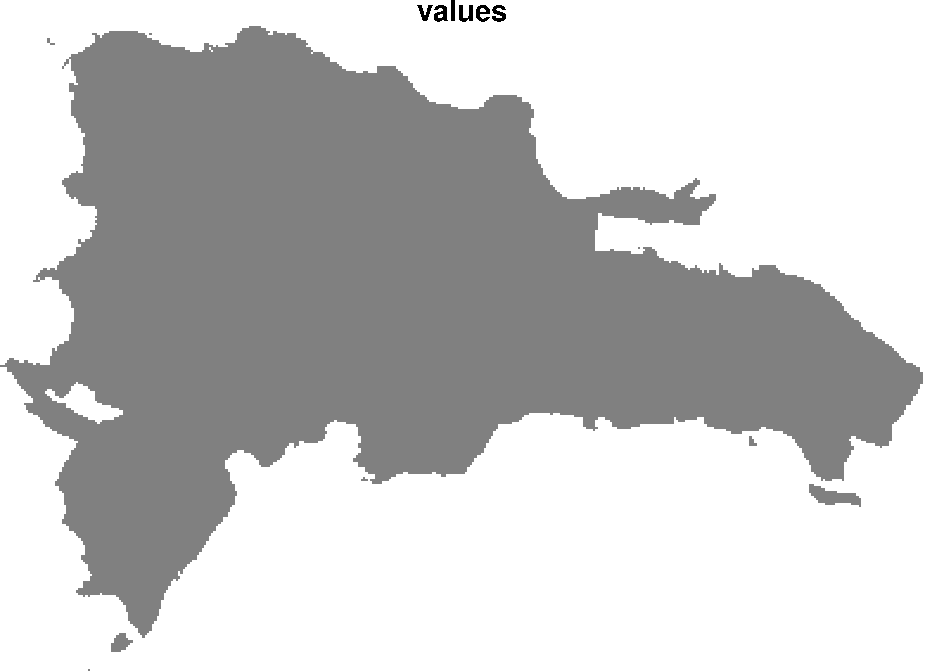
\includegraphics{proyecto_Superficie_Continua_files/figure-latex/unnamed-chunk-9-1.pdf}

Sobre esta superficie continua la cual es parte de nuestro objetivo
principal para lo que queremos lograr mas adelante , ejecutamos la
interpolación por kriging ordinario.

\begin{Shaded}
\begin{Highlighting}[]
\NormalTok{k <-}\StringTok{ }\KeywordTok{krige}\NormalTok{(}\DataTypeTok{formula =}\NormalTok{ a1998log}\OperatorTok{~}\DecValTok{1}\NormalTok{, }\DataTypeTok{locations =}\NormalTok{ pre1998, }\DataTypeTok{newdata =}\NormalTok{ grd, }\DataTypeTok{model =}\NormalTok{ f98_m2)}
\end{Highlighting}
\end{Shaded}

\begin{verbatim}
## [using ordinary kriging]
\end{verbatim}

\begin{Shaded}
\begin{Highlighting}[]
\NormalTok{k}
\end{Highlighting}
\end{Shaded}

\begin{verbatim}
## stars object with 2 dimensions and 2 attributes
## attribute(s):
##    var1.pred       var1.var     
##  Min.   :6.57    Min.   :0.00   
##  1st Qu.:7.33    1st Qu.:0.11   
##  Median :7.33    Median :0.11   
##  Mean   :7.33    Mean   :0.11   
##  3rd Qu.:7.33    3rd Qu.:0.11   
##  Max.   :7.96    Max.   :0.11   
##  NA's   :58017   NA's   :58017  
## dimension(s):
##   from  to  offset delta                       refsys point values    
## x    1 390  182216  1000 +proj=utm +zone=19 +datum...    NA   NULL [x]
## y    1 272 2205216 -1000 +proj=utm +zone=19 +datum...    NA   NULL [y]
\end{verbatim}

\begin{Shaded}
\begin{Highlighting}[]
\KeywordTok{plot}\NormalTok{(k)}
\end{Highlighting}
\end{Shaded}

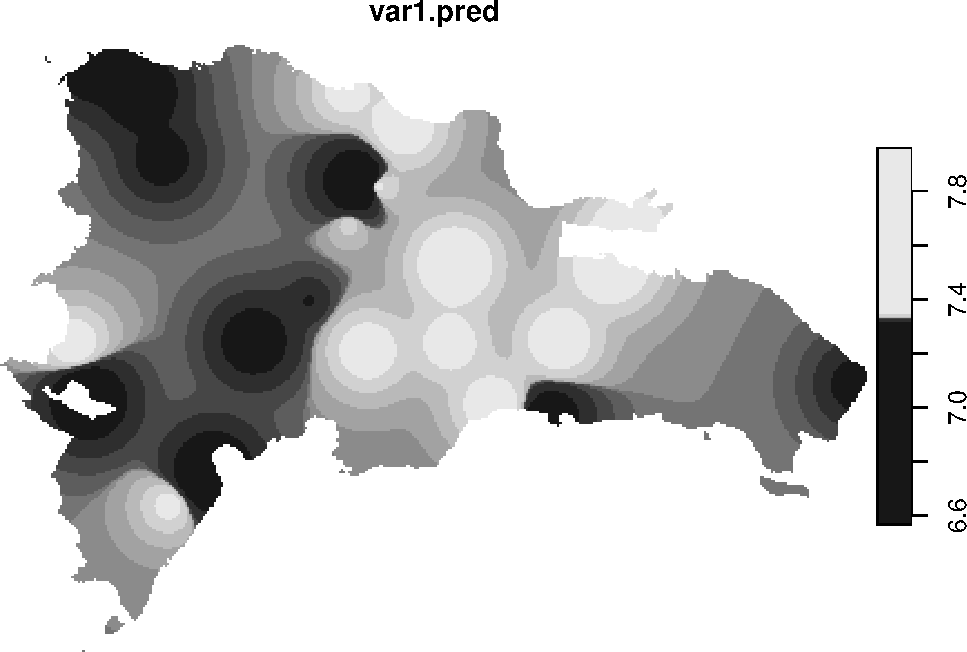
\includegraphics{proyecto_Superficie_Continua_files/figure-latex/unnamed-chunk-10-1.pdf}

\begin{Shaded}
\begin{Highlighting}[]
\KeywordTok{summary}\NormalTok{(}\KeywordTok{exp}\NormalTok{(}\KeywordTok{as.vector}\NormalTok{(k}\OperatorTok{$}\NormalTok{var1.pred)))}
\end{Highlighting}
\end{Shaded}

\begin{verbatim}
##    Min. 1st Qu.  Median    Mean 3rd Qu.    Max.    NA's 
##   711.5  1525.8  1527.5  1530.1  1530.7  2862.7   58017
\end{verbatim}

\subsection{Isoyetas}\label{isoyetas}

\begin{Shaded}
\begin{Highlighting}[]
\KeywordTok{plot}\NormalTok{(raster}\OperatorTok{::}\KeywordTok{raster}\NormalTok{(}\StringTok{'kriging.tif'}\NormalTok{))}
\KeywordTok{plot}\NormalTok{(raster}\OperatorTok{::}\KeywordTok{rasterToContour}\NormalTok{(}\KeywordTok{exp}\NormalTok{(raster}\OperatorTok{::}\KeywordTok{raster}\NormalTok{(}\StringTok{'kriging.tif'}\NormalTok{)), }\DataTypeTok{levels =}\KeywordTok{seq}\NormalTok{(}\DecValTok{600}\NormalTok{,}\DecValTok{3000}\NormalTok{,}\DecValTok{100}\NormalTok{)), }\DataTypeTok{add=}\NormalTok{T)}
\end{Highlighting}
\end{Shaded}

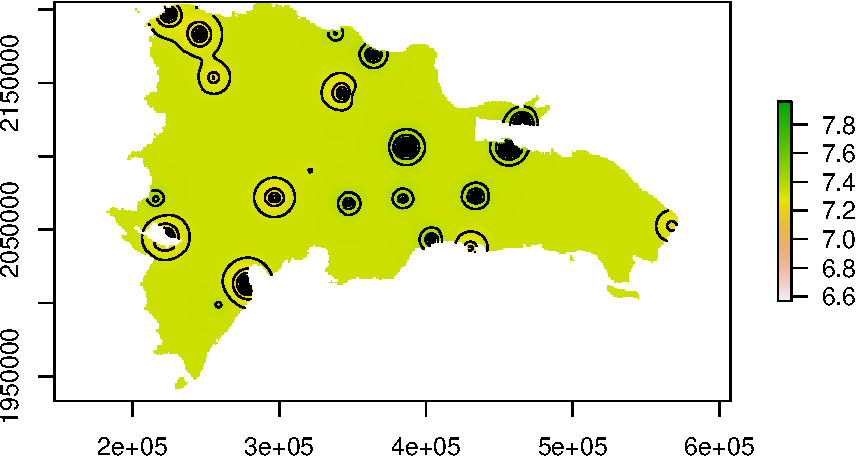
\includegraphics{proyecto_Superficie_Continua_files/figure-latex/unnamed-chunk-11-1.pdf}

\section{Representacion del objeto.}\label{representacion-del-objeto.}

\begin{Shaded}
\begin{Highlighting}[]
\KeywordTok{ggplot}\NormalTok{() }\OperatorTok{+}
\StringTok{  }\KeywordTok{geom_stars}\NormalTok{(}\DataTypeTok{data =}\NormalTok{ k, }\KeywordTok{aes}\NormalTok{(}\DataTypeTok{fill =} \KeywordTok{exp}\NormalTok{(var1.pred), }\DataTypeTok{x =}\NormalTok{ x, }\DataTypeTok{y =}\NormalTok{ y)) }\OperatorTok{+}\StringTok{ }
\StringTok{  }\KeywordTok{scale_fill_gradient}\NormalTok{(}\DataTypeTok{low=}\StringTok{"#deebf7"}\NormalTok{, }\DataTypeTok{high=}\StringTok{"#3182bd"}\NormalTok{, }\DataTypeTok{trans=}\StringTok{'log1p'}\NormalTok{) }\OperatorTok{+}
\StringTok{  }\KeywordTok{geom_sf}\NormalTok{(}\DataTypeTok{data =} \KeywordTok{st_cast}\NormalTok{(prov, }\StringTok{"MULTILINESTRING"}\NormalTok{)) }\OperatorTok{+}
\StringTok{  }\KeywordTok{geom_sf}\NormalTok{(}\DataTypeTok{data =}\NormalTok{ pre1998) }\OperatorTok{+}
\StringTok{  }\KeywordTok{geom_sf_text}\NormalTok{(}\DataTypeTok{data =}\NormalTok{ prov, }\KeywordTok{aes}\NormalTok{(}\DataTypeTok{label=}\NormalTok{TOPONIMIA), }\DataTypeTok{check_overlap =}\NormalTok{ T, }\DataTypeTok{size =} \DecValTok{2}\NormalTok{) }\OperatorTok{+}
\StringTok{  }\KeywordTok{theme_bw}\NormalTok{()}
\end{Highlighting}
\end{Shaded}

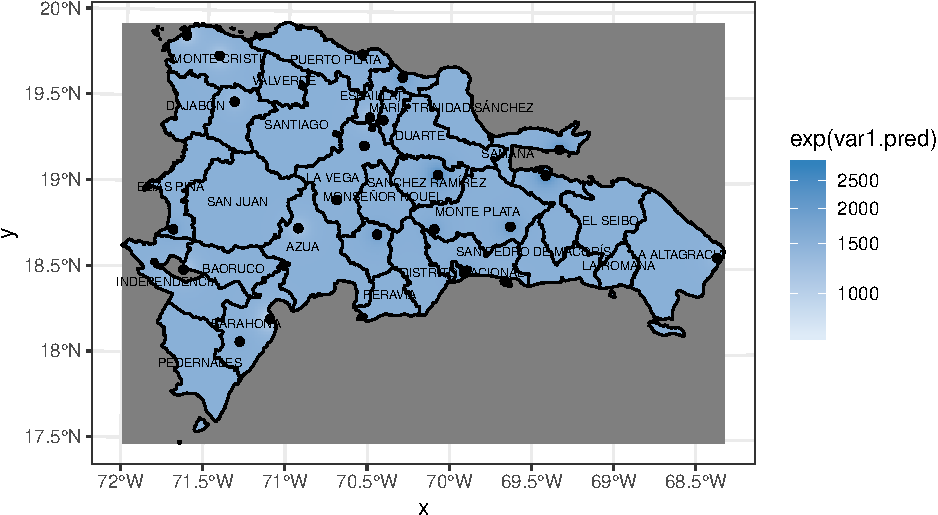
\includegraphics{proyecto_Superficie_Continua_files/figure-latex/unnamed-chunk-12-1.pdf}

\subsection{Discusión o Conclusiones}\label{discusiuxf3n-o-conclusiones}

Mediante el procedimiento utilizado para hacer los analisis de datos
puntuales y geoestadistica, aprendimos a modelisar variogramas
muestrales visualizando el comportamiento de homogeneidad de los datos
de precipitacion para el año 1998. generamos el kriging ordinario para
luego obtener una superficie continua. la cual nos da la posibilidad de
crear un mapa de curvas de lluvias o mejor dicho mapa de isoyetas. al
final de este proyecto pudimos

\ldots

\section{Información de soporte}\label{informaciuxf3n-de-soporte}

Codigos, procedimientos de la clase de superficie continua del profesor
Jose Ramon Martinez Batlle.

\ldots

\section{\texorpdfstring{\emph{Script}
reproducible}{Script reproducible}}\label{script-reproducible}

\ldots

\section{Referencias}\label{referencias}

Material de apoyo, suministrado por el profesor Jose Ramon Martinez
Batlle. Capa de division de Provincia de La ONE. (Oficina Nacional de
Estadisticas) Datos de lluvia ONAMET.(Oficina Nacional de Meteorologia)




\newpage
\singlespacing 
\end{document}
